%% Copernicus Publications Manuscript Preparation Template for LaTeX Submissions
%% ---------------------------------
%% This template should be used for copernicus.cls
%% The class file and some style files are bundled in the Copernicus Latex Package, which can be downloaded from the different journal webpages.
%% For further assistance please contact Copernicus Publications at: production@copernicus.org
%% https://publications.copernicus.org/for_authors/manuscript_preparation.html

%% copernicus_rticles_template (flag for rticles template detection - do not remove!)

%% Please use the following documentclass and journal abbreviations for discussion papers and final revised papers.

%% 2-column papers and discussion papers
\documentclass[, manuscript]{copernicus}



%% Journal abbreviations (please use the same for discussion papers and final revised papers)


% Advances in Geosciences (adgeo)
% Advances in Radio Science (ars)
% Advances in Science and Research (asr)
% Advances in Statistical Climatology, Meteorology and Oceanography (ascmo)
% Annales Geophysicae (angeo)
% Archives Animal Breeding (aab)
% ASTRA Proceedings (ap)
% Atmospheric Chemistry and Physics (acp)
% Atmospheric Measurement Techniques (amt)
% Biogeosciences (bg)
% Climate of the Past (cp)
% DEUQUA Special Publications (deuquasp)
% Drinking Water Engineering and Science (dwes)
% Earth Surface Dynamics (esurf)
% Earth System Dynamics (esd)
% Earth System Science Data (essd)
% E&G Quaternary Science Journal (egqsj)
% Fossil Record (fr)
% Geochronology (gchron)
% Geographica Helvetica (gh)
% Geoscience Communication (gc)
% Geoscientific Instrumentation, Methods and Data Systems (gi)
% Geoscientific Model Development (gmd)
% History of Geo- and Space Sciences (hgss)
% Hydrology and Earth System Sciences (hess)
% Journal of Micropalaeontology (jm)
% Journal of Sensors and Sensor Systems (jsss)
% Mechanical Sciences (ms)
% Natural Hazards and Earth System Sciences (nhess)
% Nonlinear Processes in Geophysics (npg)
% Ocean Science (os)
% Primate Biology (pb)
% Proceedings of the International Association of Hydrological Sciences (piahs)
% Scientific Drilling (sd)
% SOIL (soil)
% Solid Earth (se)
% The Cryosphere (tc)
% Web Ecology (we)
% Wind Energy Science (wes)


%% \usepackage commands included in the copernicus.cls:
%\usepackage[german, english]{babel}
%\usepackage{tabularx}
%\usepackage{cancel}
%\usepackage{multirow}
%\usepackage{supertabular}
%\usepackage{algorithmic}
%\usepackage{algorithm}
%\usepackage{amsthm}
%\usepackage{float}
%\usepackage{subfig}
%\usepackage{rotating}


% The "Technical instructions for LaTex" by Copernicus require _not_ to insert any additional packages.
%


\begin{document}

\title{Monitoring seasonal wheat growth across northern India, a Picture Based
Insurance crop monitoring dataset}


\Author[1]{Koen}{Hufkens}
\Author[2]{Francisco}{Ceballos}
\Author[3]{Timothy}{Foster}
\Author[4]{Michael}{Mann}
\Author[2]{Miguel}{Robles}
\Author[5]{Mann Singh}{Toor}
\Author[2]{Berber}{Kramer}


\affil[1]{Department of Applied Ecology and Environmental Biology, Ghent
University, Belgium}
\affil[2]{Markets, Trade, and Institutions Division, International Food Policy
Research Institute, Washington DC, USA}
\affil[3]{School of Mechanical, Aerospace and Civil Engineering, University of
Manchester, Manchester, UK}
\affil[4]{Department of Geography, The George Washington University, Washington
DC, USA}
\affil[5]{Department of X}

%% The [] brackets identify the author with the corresponding affiliation. 1, 2, 3, etc. should be inserted.



\runningtitle{running title}

\runningauthor{Hufkens et al.}


\correspondence{Berber\ Kramer\ (b.kramer@cgiar.org)}



\received{}
\pubdiscuss{} %% only important for two-stage journals
\revised{}
\accepted{}
\published{}

%% These dates will be inserted by Copernicus Publications during the typesetting process.


\firstpage{1}

\maketitle


\begin{abstract}
We present a consistently processed dataset of (\textasciitilde{}20K)
near-surface remote sensing crop images acquired using inexpensive
smartphones of 1685 smallholder farmers fields in northwest India.
Monitoring crop growth and disturbances, for instance for crop insurance
applications, is critical for targeting interventions to support farmers
to manage and mitigate production risks. Presented smartphone images
monitored winter wheat growth and includes meta-data, either manually or
automatically derived, to quantify crop greenness, phenology and damage
events as well as management practices. Our dataset offers granular
visual field data, providing detailed information on the timing of key
developmental phases of winter wheat and crop growth disturbances which
are not registered by common satellite remote sensing vegetation indices
or national crop cut surveys. Our high-resolution dataset provides a
rich source of inputs that can be used to improve crop yield and
production risk estimation in smallholder agricultural systems.
Keywords: crowdsourcing, remote sensing, winter wheat, insurance, India
\end{abstract}




\introduction[Introduction]

Smallholder agriculture supports livelihoods of 2.5 billion people
globally, contributing 30-50\% of global food supply and 80\% of the
food produced in Sub-Saharan Africa and Asia
\citep{ifad2013, lowder2016}. Although smallholder agriculture underpins
food security, the scale at which smallholder farmers operate make them
highly vulnerable to production risks resulting from localized extreme
weather events.

Agricultural advisory services and crop insurance can help farmers
manage these risks, but the quality of these services will crucially
depend on the ability to monitor extreme weather events and their
impacts on crop development. In that regard, it is important to note
that the impact the impact of extreme weather events is not distributed
equally. Differences in socio-economic background and the highly
localized nature of some extreme weather events (e.g.~heavy rainfall,
hailstorms) can result in heterogeneous crop losses even within small
geographic areas \citep{below2012, fishman2016, ifad2013, jain2015}.
Extreme weather events are likely to be exacerbate through climate
change, both in terms of their frequency and magnitude, across both
tropical and sub-tropical regions where most smallholder farmers are
concentrated \citep{auffhammer2012, harvey2014, morton2007}. This
highlights the urgent need for solutions to improve producers'
resilience to weather-related production risks throughout the growing
season.

For example, heat stress has damaging impacts on yields especially
during crop flowering, or anthesis \citep{lobell2011}. Temperatures
above 30\(^\circ\)C during wheat anthesis cause complete sterility
\citep{farooq2011, saini1982}. Lodging of wheat through the toppling of
stems is known to be heavily influenced by occurrence of heavy rain
and/or high wind only in later stages of wheat development
\citep{berry2003, gent1997, vera2012}. Both examples highlight the
importance of monitoring crop development (or phenology) at an
appropriate scale across time. Measurements of crop phenology are
therefore critical inputs to support monitoring of agricultural
productivity in smallholder systems and provide targeted interventions
\citep{auffhammer2012, carletto2015, harvey2014, morton2007}.

To date, efforts to monitor and map weather impacts on production have
been limited by a lack of systematic field-level crop (yield) data
collection and reporting (e.g.~via farmer surveys) in most developing
countries. Similarly, while advances have been made in the use of remote
sensing imagery to map crop yields at field-scales
\citep{azzari2017, burke2017, jain2015}, there remain significant
challenges to the application of satellite-based methods for reliable
crop yield assessment in smallholder systems due to the mismatch between
the spatial resolution of openly-accessible satellite imagery, small
plot sizes, highly heterogeneous cropping patterns, and high levels of
cloud cover during crop growth seasons
\citep{duncan2015, jain2017, mann2017, hufkens2019}. However, there is a
potential to use near-surface imagery, i.e.~conventional digital images
taken near ground level, to support phenological monitoring and rapid
assessments of field-level impacts of extreme weather events on
smallholder agricultural productivity \citep{hufkens2019, ceballos2019}.
Previous research has shown that near-surface imagery of crop
\citep{hufkens2019} and vegetation \citep{hufkens2012} development has
the ability to capture growth phases at a scale which is not attainable
using medium to high resolution satellite remote sensing data. More so,
the visual nature of the data allows for intuitive post-hoc assessments
of crop damage and growth stages in support of classical statistical and
machine learning based analysis.

Here, we describe a curated dataset of georeferenced and time-stamped
smartphone images of insured wheat fields originally collected to
support insurance claims verification, or Picture Based Insurance (PBI)
\citep{ceballos2017}, across two winter growing seasons (Rabi) in
India's Punjab and Haryana states. Given the strong dependence of crop
yields on intra-seasonal weather variability and management practices,
these data and their derived data products could enable significant
improvements in field-level crop growth status and yield loss estimation
in agricultural systems, as well as remote sensing product validation.

\section{Study location}

The study summarized data from two separate field trials across two
Rabi, across India's Punjab (Fatehgarh, Ludhiana, Patiala districts) and
Haryana (Fatehabad, Sirsa, Yamunanagar districts). These states are part
of the Indo-Gangetic Plains, a zone of importance for crop production,
which accounts for around 30\% of India's total wheat production.

The climate across both states is mostly dominated by a hot arid steppe
climate, according to the Koeppen-Geigen scale. The southern part of
both states are characterized by warm temperate conditions with dry
winters and hot summers, while the north has an arid hot desert climate.
Most of the villages in our field trials were located in a hot arid
steppe climate. Smallholder agriculture in this area is largely
mechanized and is heavily reliant on irrigation \citep{kumar2018}.
Punjab and Haryana fields are typically double-cropped with rice (or
cotton) planted during the Kharif monsoon (June - October), and wheat
planted in the Rabi season (October - March). Across all sites, mean
annual temperatures and precipitation are 24.45 \(\pm\) 0.2\(^\circ\)C
and 725 \(\pm\) 215 mm, respectively \citep{Hijmans2005} while
precipitation between sites varies from 315 to 1407 mm.

The PBI initiative selected study sites following a clustered sampling
approach. A 150 villages were randomly chosen within a radius of 5km
from third-party weather stations in the area. During the first Rabi 50
villages were included in the study, while we increased sampling during
second Rabi adding and additional 100 villages. Within each village, 15
farmers satisfying a number of criteria were randomly selected to be
invited for study participation. The criteria required
\citep{ceballos2019} that the smallholder farmer (1) had less than 15
acres of operational land; (2) was in possession of an android
smartphone; and (3) was planning to grow wheat during the upcoming
growing season (running from November - April). Over two growing seasons
a total of 1685 farmers (or 4 \(\pm\) 4 farmers per village) agreed to
participate in the PBI studies. For these farmers, the study team listed
all plots on which the farmer was planning to grow wheat, and randomly
selected one field for each farmer to be included in the study. Image
acquisition in the first-year villages was coordinated by the Borlaug
Institute for South Asia and the new second-year villages in Haryana
were suppervised by the Centre for Agriculture and Bioscience
International (CABI) and its subcontractor Kisan Sanchar.

\section{Data acquisition \& Screening}

During the first field season farmers were asked to take 1 -- 3 repeat
pictures per week throughout the season, between 10:00h and 14:00h local
time from approximately the same location as an initial northward
oriented picture, and with approximately the same viewing angle. During
the second field season data acquisitions were lowered to a suggested
image every 4 days. The outlined protocol adheres as closely as possible
to the PhenoCam guidelines established by \citet{Sonnentag2012}, while
taking into consideration the constraints imposed by the use of a
smartphone and the farmer's time availability. Image acquisitions were
facilitated using a custom Android application (WheatCam).

The farmer set up an observation site by taking an initial
geo-referenced image of a field. Subsequent images were referenced
relative to the initial ``ghosted'' image (a mildly transparent image of
the initial picture) and the location shown on an interactive map.

The application allowed the farmer to frame nearly identical repeat
pictures relative to landscape features (or one or two installed
reference poles, which were used only in the first year). A fixed white
balance between images was used to minimize in-camera adjustment of
illumination and RGB ratios. All pictures were uploaded to a server for
further processing.

Before further processing we manually screened all images to ensure that
no people were present in the image scenes, to guarantee their privacy.
In addition, we removed images which were mistakenly taken indoors, or
other accidental acquisitions. We further screened for images which were
excessively blurred or discoloured, covered by a finger or otherwise not
contained little vegetation or taken during crop cutting or application
development.

We anonymized the dataset by masking most non-vegetation details which
might provide clues to the exact position of a farmers' field, while
selecting the vegetation of interest for processing (see below). In our
dataset we provide all images anonymized sorted by farmer, as indicated
by a sequential number (see data descriptor below).

\begin{figure}
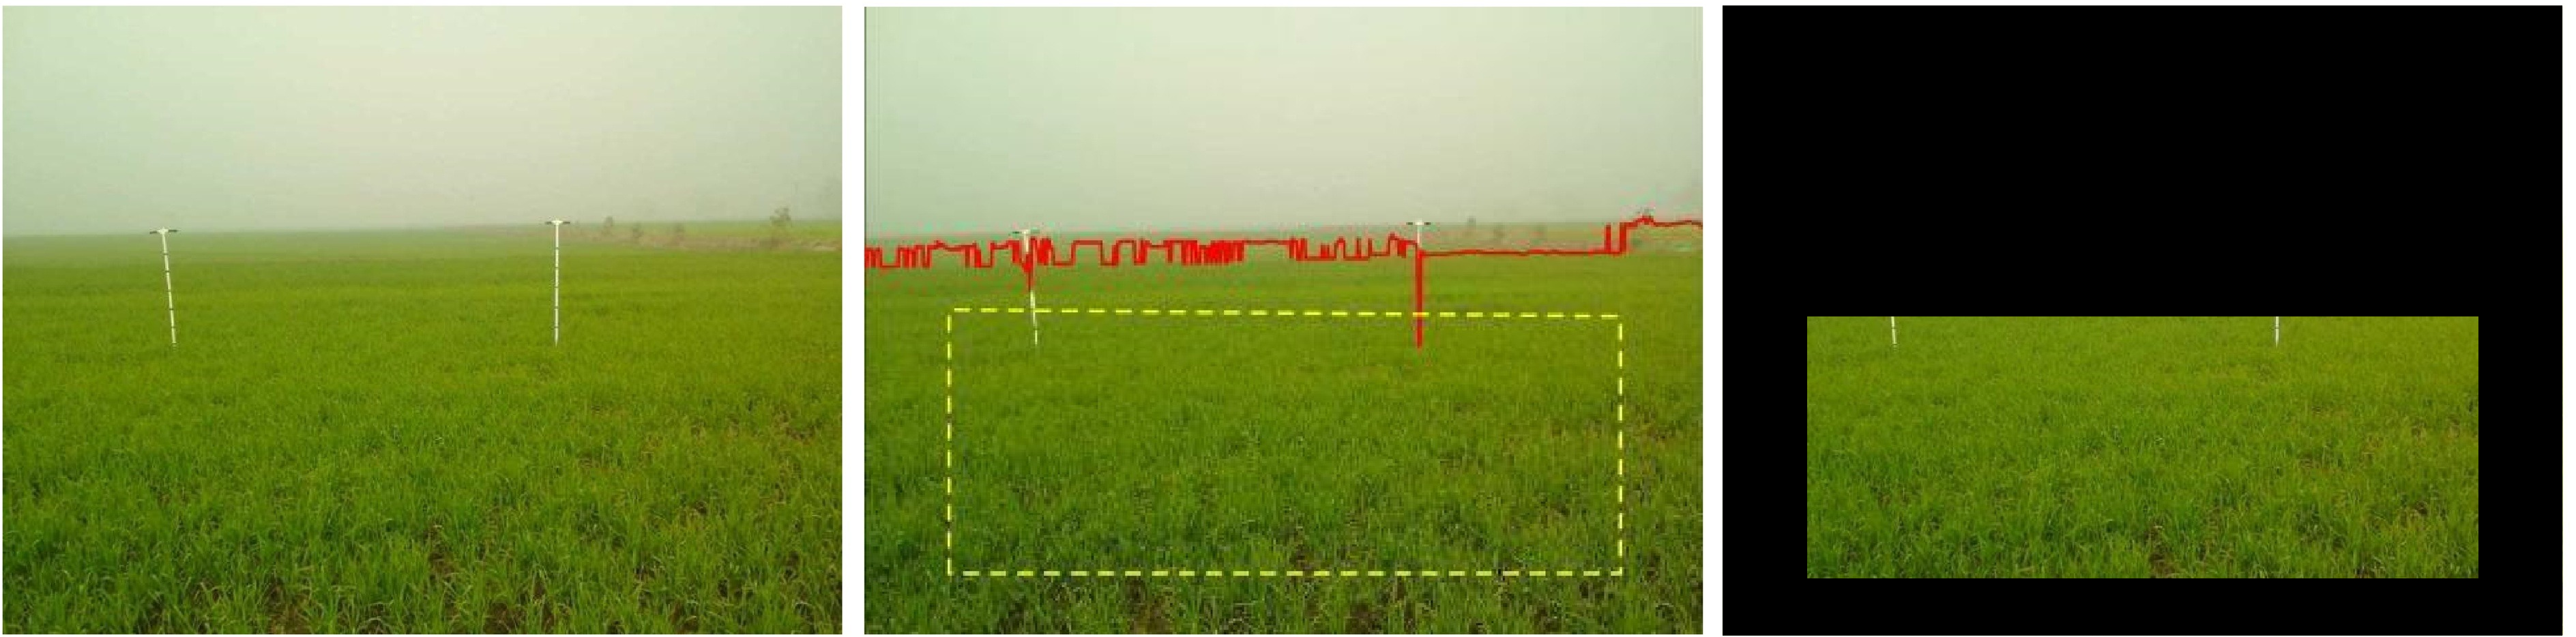
\includegraphics[width=16cm]{./figures/image_processing} \caption{Image as acquired by a smallholder farmer of a wheat field during the early growing season (left panel). The location of image acquisition location was constrained by the reference pole(s) in the image and the GPS location of the farmer's smartphone. The image was anonymized by automatically detecting the approximate horizon (center panel) to define a region of interest, which is retained while all other data is set to black (right panel), limiting identifiable landscape elements. Image adapted from [@hufkens2019]}\label{fig:unnamed-chunk-1}
\end{figure}

\section{Preprocessing}

\subsection{Region-of-Interest delineation \& privacy measures}

It has been shown that greenness indices calculated from digital repeat
photography provides valuable information on the phenology of natural
ecosystems and agricultural fields alike
\citep{richardson2018, hufkens2016, hufkens2019}. However, most digital
repeat photography uses fixed tower based cameras, making image
processing relatively straightforward using a fixed Region-of-Interest
(ROI) over which to calculate greenness metrics. The absence of a fixed
vantage point made delineating a fixed ROI over which to calculate this
color vegetation index impossible. We therefore automatically delineate
a ROI on an image-by-image basis using a horizon detection algorithm.
The algorithm first resizes the image to 640 pixels along the x-axis,
scaling the y-axis proportionally. The algorithm finds change points in
the blue channel along the vertical axis of the images using the Pruned
Exact Linear Time (PELT) method \citep{killick2011}, approximating the
location of the horizon. We then define a trapezoid ROI defined by the
median horizon locations for the left and right half of the image,
padded by 15\% of the image height and 10\% of the image width along y
and x-axis directions respectively. Similarly, the two bottom corner
points were defined by padding the bottom and sides of the image by 10\%
of the image width and height. We use this ROI to exclude most other
features from the original image which do not pertain to the area
evaluated. Areas of no interest are set to black and the image is saved
to disk. In addition, we manually screened all processed images and made
manual corrections to guarantee the privacy of volunteer farmers where
necessary.

\subsection{Vegetation indices}

We calculated a number of vegetation indices for every images based upon
band ratios of the red, green and blue channel image data (i.e digital
numbers or DN). In particular, we calculated the 90\textsuperscript{th}
percentile Green Chromatic Coordinates (Gcc, Eq. 1) across the ROI of
every image to increase the stability of the greenness signal over time
\citep{Sonnentag2012, richardson2018}. Gcc is defined as the ratio of
the green digital number and the sum of all digital numbers (or image
brightness, see Eq. 1).

Smartphone cameras are not radiometrically calibrated. Absolute Gcc
values are therefore affected by differences in image rendering between
devices, making the absolute values incomparable across sites. As such,
Gcc values were composed into time series smoothed and normalized
between 0 and 1 using a fitted locally estimated scatterplot smoothing
(loess) model with a fixed span of 0.4. Normalization between 0 and 1
accounts for these differences in image rendering and allows us to
create data that is meaningfully comparable. Smoothing of the Gcc time
series removes occasional outliers but retains the overall trajectory,
when sufficient data points are available. Due to uneven time steps in
image acquisition we use daily interpolated smoothed data in all
subsequent analyses and data products. If insufficient data is
available, the smoothing routine will effectively be a linear
interpolation between data points. Both the original values and the
normalized smoothed data for acquisition dates are reported in our
dataset.

\begin{verbatim}
  Gcc = Green DN / (Red DN + Green DN + Blue DN)            (Eq. 1)
\end{verbatim}

We also report the 90\textsuperscript{th} percentile Red Chromatic
Coordinate (Rcc, Eq. 2) and the 10\textsuperscript{th} percentile Green
Red Vegetation Index (GRVI, Eq. 3, \citet{motohka2010}) and the
individual DN of the three (RGB) colour channels. These data allow for
further analysis of the colour information in the images without the
reprocessing of the image data.

\begin{verbatim}
  Rcc = Red DN / (Red DN + Green DN + Blue DN)          (Eq. 2)
  GRVI = (Green DN - Red DN) / (Red DN + Green DN)          (Eq. 3)
\end{verbatim}

\subsection{Ancillary data}

Before and during the image acquisition farmers were asked to complete a
survey on crop varieties used, management practices applied and damages
sustained. We report the variety of wheat planted, the presence of
irrigation, the application of fertilizer, pesticides or herbicides
since the last image taken. Statistics are provided on an image by image
basis. Synoptic overviews of these data are provided in the spatially
aggregated summary products (see below).

Both field trials had different survey inputs concerning wheat
development assessments. For consistency, we aggregated these into the
common Zadoks scale of wheat growth stages \citep{zadoks1974} using a
reclassification key or ontogeny (Table 1). We assigned values 0 and 10
to land preparation and post harvest phases, respectively, which did not
fit the standard wheat development scale.

Note that wheat development phases during the first growing season were
assessed by agronomists. In contrast, wheat development phases of the
second growing season were self-reported, introducing considerable
uncertainty. Discrepancies exist due to misinterpretation of these
growth phases by the farmers.

\begin{table}[ht]
\centering
\caption{Translation key for reclassification of manual labels across the two growing seasons (Rabi) into the Zadoks scale of wheat development.} 
\begin{tabular}{llrr}
  \hline
Rabi 2016 - 2017 & Rabi 2017 - 2018 & Zadoks & Non Zadoks (out of range) \\ 
  \hline
 Land Preparation Phase &  &  &   0 \\ 
   & Crown root &   1 &  \\ 
  Early Vegetative Phase & Tillering &   2 &  \\ 
  Mid Vegetative Phase &  &   3 &  \\ 
  Late Vegetative Phase & Booting &   4 &  \\ 
  Flowering and Reproductive Phase & Heading &   5 &  \\ 
   & Anthesis &   6 &  \\ 
  Ripening and Maturity Phase & Milking &   7 &  \\ 
  Post Harvest Phase &  &  &  10 \\ 
   \hline
\end{tabular}
\end{table}

\section{Post-processing \& derivative data products}

\subsection{Data product structure}

Our final data products consists of four main parts (1) the anonymized
image data, (2) a master file of data derived from the individual images
combined with matching ancillary data, (3) a summary dataset providing
an overview of the data by regional aggregation derived, and finally,
(4) a data file containing smoothed time series by regional aggregation.
The latter two products are derived from the master file and are
provided for convenience in a format to reach a broad audience while
limiting the processing by the end user.

To limit the number of files, at the expense of file size, we include
all field based quality control summary data into the master data file.
Summary statistics based upon the aggregated spatial units were used to
anonymize the data. These summaries provide insights into regionally
averaged trends and include for example the number of farmers who
reported irrigation or other management practices for a given town or
WorldClim grid cells. These two formats are provided as aggregated
levels will appeal to different research diciplines. We used two
aggregation approaches as administrative boundaries are more meaningful
in socio-economic analysis and gridded data are more relevant within the
context of remote sensing validation and crop modelling.

To support easy processing in both R or using the python (pandas)
environments we structured all data according to tidy data principles
\citep{wickham2014}, or row first (long format) orientation. Detailed
lists of variables and the data structures are provided in the Appendix
tables 1 to 3, while a full description of the post-processing and
summary statistics routines is provided below.

\subsection{Geospatial anonymization}

The data were anonymized by aggregating the exact field locations to
larger spatial units. These spatial units ensures a suitable level of
obfuscation to provide the volunteer smallholder farmers with the
required privacy. In order to accommodate several use cases all data
locations (coordinates) are anonymized using either administrative
boundaries or common grid cell spacing used in climate products. The
final (master) dataset, as such, does not contain any geo-location data
of individual farmers, to maintain their privacy, while retaining some
spatial information to support subsequent spatial analysis. We used the
publicly available India Village-Level Geospatial Socio-Economic Data
Set (SEDAC, accessed January 2020) to re-assign field locations to the
centroid of the village polygon. Similarly, we used the WorldClim
\citep{Hijmans2005} grid cell layout to provide grid cell locations at
both a 2.5 and 5 minute grid levels. Combined with the removal of most
recognizable features in the raw image data (see above) these spatial
untis ensure the privacy of the volunteers.

\subsection{Quality control}

We provide several ways to screen data for quality in acquisition
frequency and timing. We include the number of images for each field,
the duration of the acquisitions (in days), the mean spread between
individual image acquisitions and a derived quality assurance (QA)
index. The QA index is defined as the ratio between the total image
count and the spread.

\begin{verbatim}
  QA = Total number of acquired images / days between acquisitions (Eq. 4)
\end{verbatim}

The lower the QA index, the lower the quality of the resulting time
series of images. The QA index, and other quality control data allows
for the screening of the data at both the field level and the level of
the spatial unit. These quality indicators are propagated from a field
level to spatial units level through averaging.

\subsection{Crop phenophases \& phenology time series}

We report crop phenology statistics as phenological phases (phenophases)
for all spatial locations and all spatial units (i.e.~SEDAC village
level and both WorldClim grid cell sizes). Fixed threshold values were
applied to quantify the end of the wheat tillering phase and the start
of ripening, at 73\% and 83\% of the rising and falling part of the
seasonal Gcc curve respectively. These thresholds have previously been
linked to distinct developmental phases of wheat \citep{hufkens2019}.
Both wheat phenophases, tillering and the start of ripening, approximate
Zadoks scale levels 2 and 5.

We pooled all raw Gcc data across a spatial unit. Doing so we leveraged
all available image data, rather than averaging field based phenoloy
estimates. Prior to calculating these thresholds the Gcc data is
smoothed using a loess curve with a span value of 0.4 and normalized
between 0 an 1. If insufficient data was available smoothing would
result in simple linear interpolation between data points. All phenology
metrics are reported as ISO dates (YYYY-MM-DD), with standard deviation
in days. All dates are reported irrespective of the quality of the data
on a field or aggregated level. We refer to the data QA index and
provided code for further screening of the reported data or bespoke
reprocessing. Finally, we report the smoothed normalized seasonal
profiles of crop greenness (Gcc) for all spatial locations.

\subsection{Summary statistics}

Although all raw data is reported in the master data file we provide a
number of summary statistics based on common use cases. For spatial
locations across spatial units we provide summary statistics for the
number of fields and farmers for a given spatial location as well as the
total number of fields where management practices were reported
(weeding, tilling, sowing, damages by rain etc). We report the mean and
standard deviation for those statistics which include measured values,
such as the density of fertilizer or herbicide applied (kg / acre). In
addition, quality assurance metrics are propagated and we report the
mean QA index, spread, number of values, and duration for a given
spatial location. We also provide the total number of values, and where
available the mean and standard deviation on the self-reported sowing
date. We acknowledge that we do not provide every possible summary
statistic as derived from the master data file. However, by making all
processing code available we hope to facilitate custom summary
statistics from the master data file according to bespoke needs (see
code availability).

\section{Results}

We present a consistently processed dataset of near-surface remote
sensing images acquired using inexpensive smartphones at 1697
smallholder farmers fields in northwest India (476 and 1221 for the
first and second growing season, respectively). In the interest of
brevity in reporting on the dataset we will limit summary statistics to
either global statistics across the two growing seasons or regional ones
for the SEDAC town based boundaries.

Across the two growing season, 1964 fields were monitored. A total of
20294 images were considered valid for processing. Data coverage across
sites varies widely from a couple of images acquired throughout the
entire growing season, to steady biweekly acquisitions. On average for
every field across the two seasons, 17.8 \(\pm\) 18.1 and 7.73 \(\pm\)
10.6 images were recorded for the first and second growing season,
respectively. The difference in numbers of images per field between the
two seasons can be attributed to a more relaxed requirements during the
second field season.

\begin{figure}
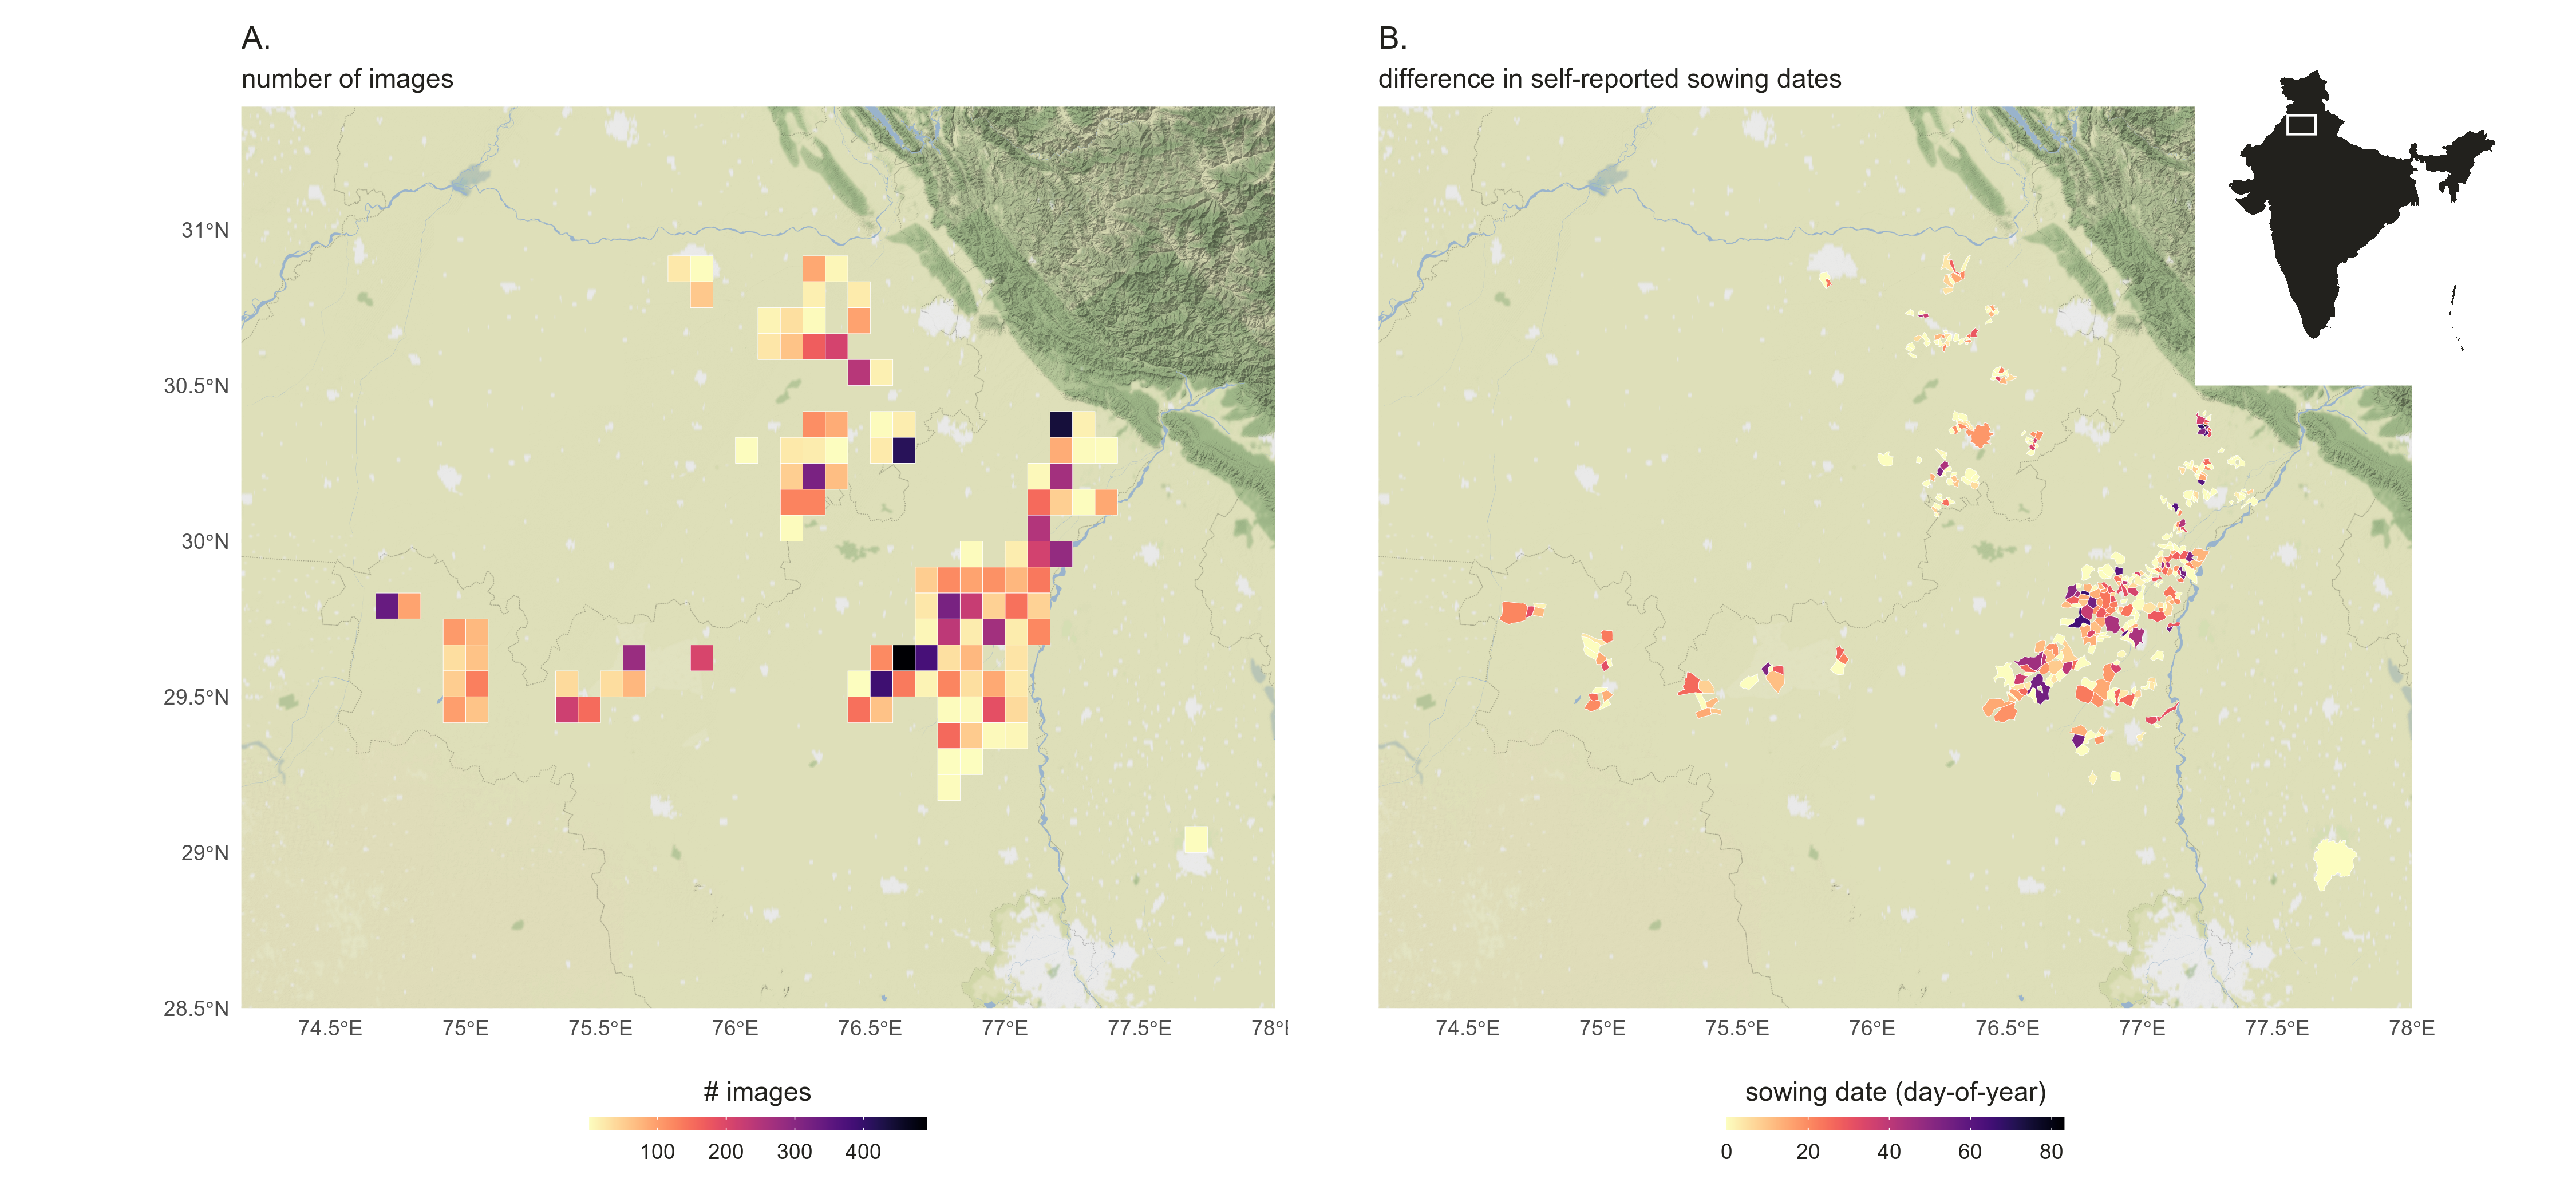
\includegraphics[width=1\linewidth]{./figures/summary_map} \caption{Summary maps of some of the data. A. The number of farmers at a WordClim 5 degree grid size and B. the difference between first and last self-reported sowing date in a given village (SEDAC polygons). Topleft inset provides the location of the plotted area within India itself. Both aggregation levels are provided in the dataset.}\label{fig:unnamed-chunk-3}
\end{figure}

Although the ancillary data was voluntarily reported, and hence uptake
of reporting might vary, some important trends could be noted. In
general irrigation is a widespread practice in the region which is
corroborated by the self-reported data, with 60 (\(\pm\) 12) \% of the
fields being irrigated at some point during the growing season.
Aggregating across various resolutions we see that throughout the region
no obvious spatial patterns exist with respect to irrigation (Figure 2),
suggesting widespread access to water sources and irrigation
infrastructure \citep{kumar2018}.

Similarly, it is shown that both the sowing dates self-reported during
the second season or the timing of tillering across all growing seasons
is widely variable across fields and regions. Evaluating the
self-reported sowing dates we find a mean sowing date of the 11th of
November, with a standard deviation of 14 days. These self-reported
statistics are in line with previously assessed dates from the first
season \citep{hufkens2019}.

\begin{figure}
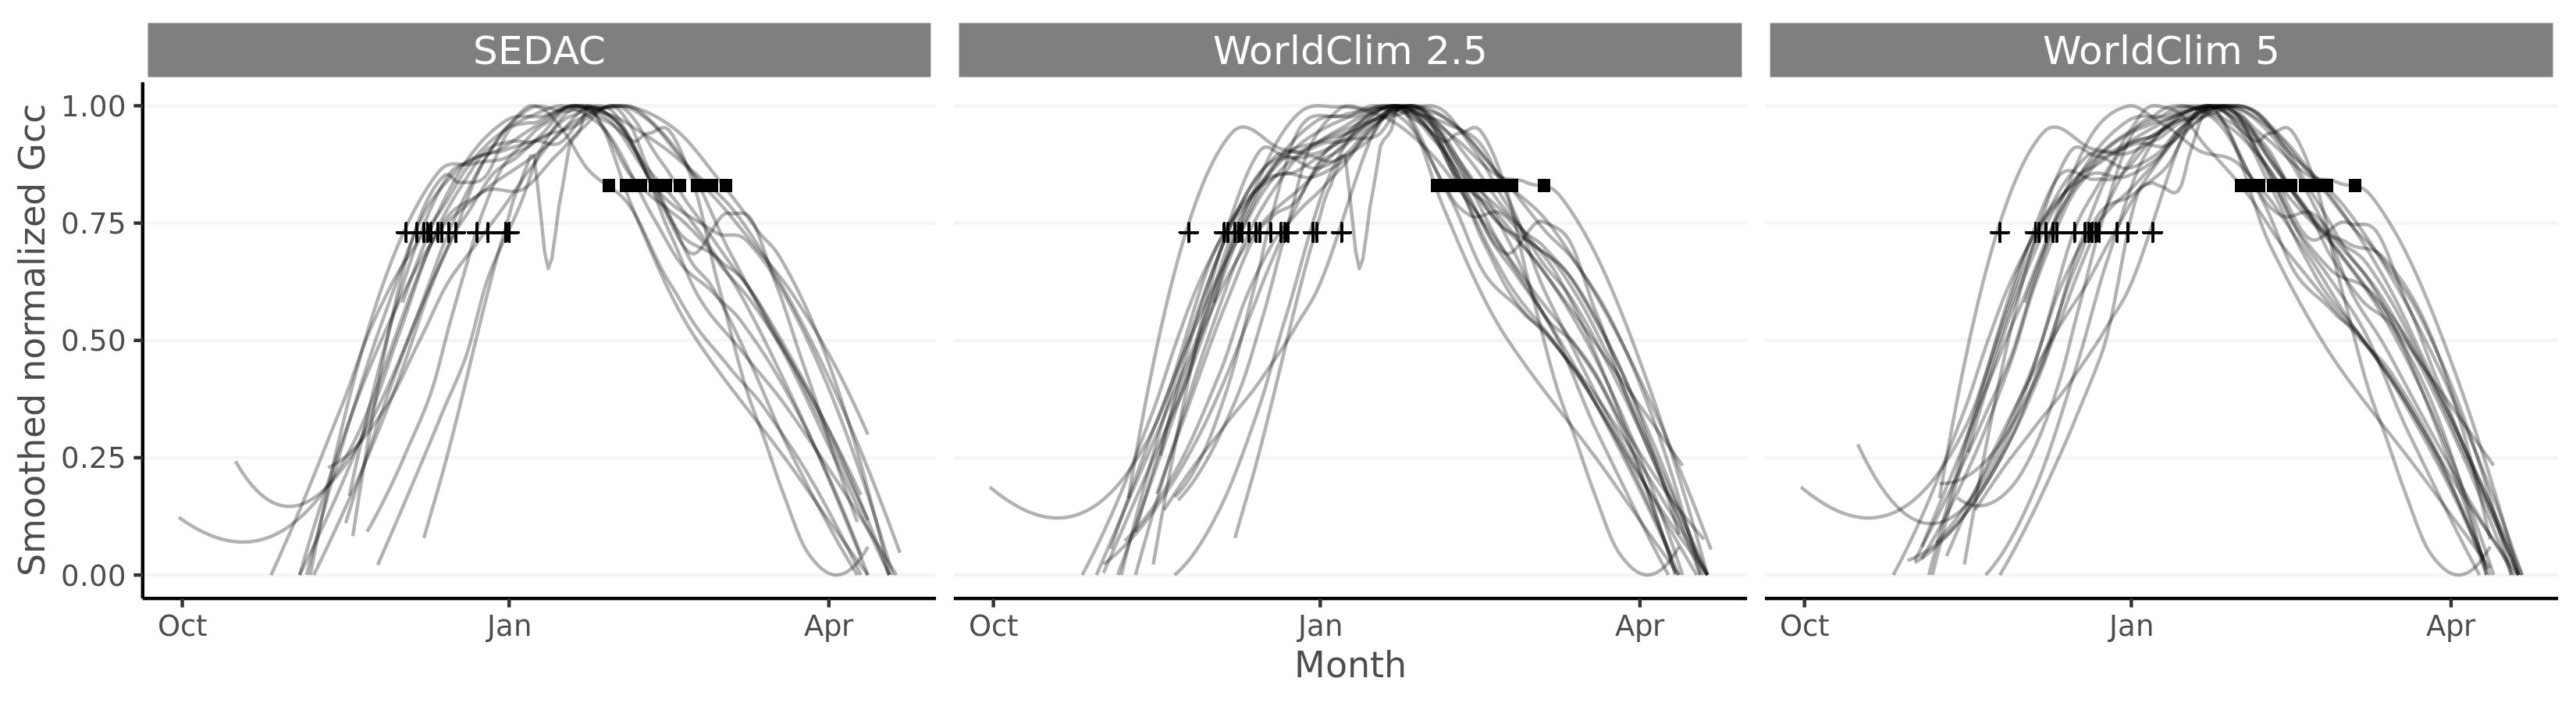
\includegraphics[width=1\linewidth]{./figures/summary_time_series} \caption{Normalized and smoothed time series of vegetation greenness (Gcc) aggregated by spatial location and spatial unit. Only spatial locations with more than 150 image acquisitions are shown. Phenology transition dates at 73 and 83 percent threshold level of the curve are depicted by a plus and square marks, respectivelly.}\label{fig:unnamed-chunk-4}
\end{figure}

There are slight differences between the two growing seasons when
comparing the phenology during the early season development (rising part
of the Gcc curve). Here, the first season is on average a month early
compared to the second growing season, reflecting differences in local
crop management practices, with threshold dates reported at the 27th of
December and the 24th of January respectively. Despite the difference in
the timing of wheat growth between both growing season the variability
within both datasets is similarly large up to 18.5 and 19.9 days, for
the first and second season respectively. Using either the first image
acquisition (a proxy for the sowing date) or the first sowing dates, for
the first and second season respectively, we observe a difference of up
to a month in the sowing of crops.

\begin{figure}
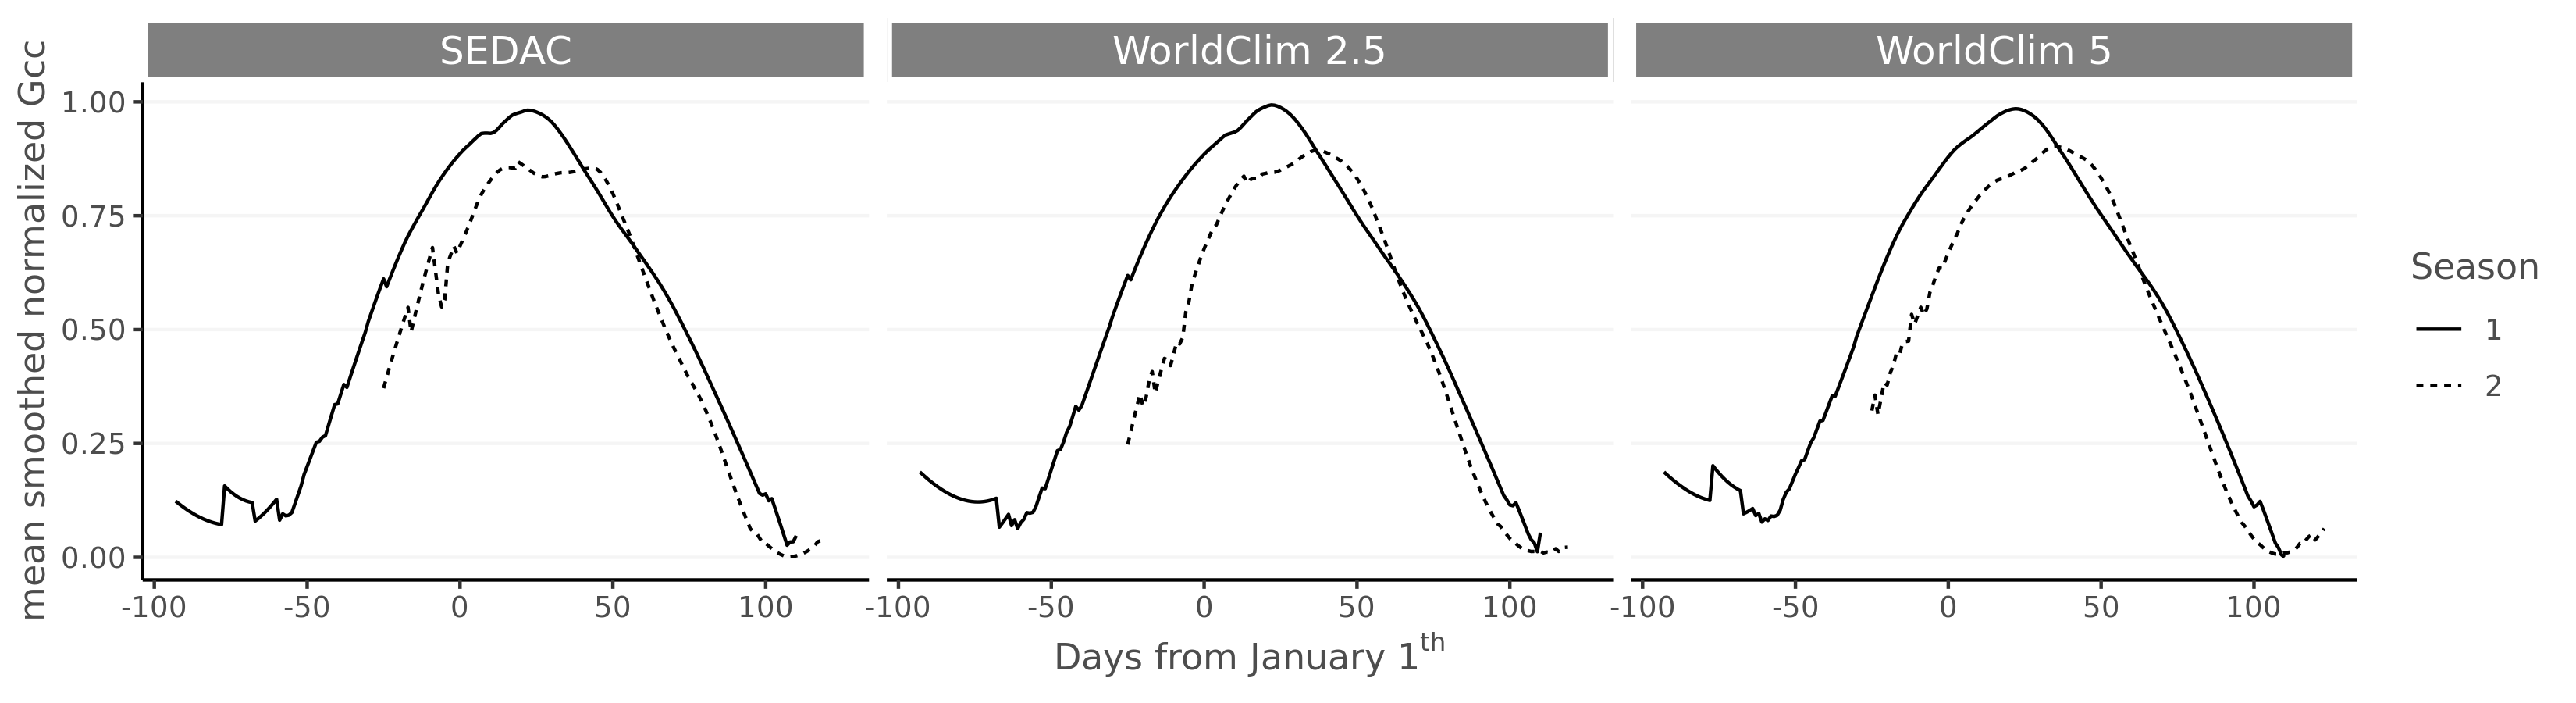
\includegraphics[width=1\linewidth]{./figures/summary_time_series_2} \caption{Average normalized and smoothed time series of vegetation greenness (Gcc) by spatial unit for both growing seasons, showing the difference in average timing of crop development. Crop development is shown relative to the first of January of the growing season. Only spatial locations with more than 150 image acquisitions are shown.}\label{fig:unnamed-chunk-5}
\end{figure}

Looking at the variability across fields we see large differences in
field management and subsequent crop development, which highlights the
value of collecting plot-level images and associated farmer reports. In
general there is large variability between fields. These differences
have consequences which potentially propagate throughout the whole
growing season, or could safeguard some farmers from crop damage while
exposing others unduly. Our dataset shows that if sufficient data is
available a clear seasonal trajectory and phenologically relevant
transition dates can be extracted. Previous research has shown that
these transition dates are linked to physiologically relevant growth
phases, making them valuable inputs for model development or remote
sensing validation \citep{hufkens2019}. Both the smoothed time series,
and the extracted phenological transition dates are therefore key
products derived from our image time series.

\section{Conclusion}

We provide an anonymized dataset which characterizes the seasonal
variability in crop development during two winter wheat growing seasons
in Northern India, based upon \textasciitilde{}20K near-surface remote
sensing images. The data presented monitored both winter wheat growth by
asking farmers to take pictures of their crops using their own
smartphone cameras and extensive farmer reported meta-data on management
practices, in addition to expert assessments on crop development and
disturbances. In addition to raw data we highlight ways to process,
anonymize and summarize the crowdsourced smartphone images, and provide
derived data products to quantify crop greenness, phenology and regional
data summaries. These data can provide valuable inputs to support crop
modelling, validation of satellite remote sensing and machine learning
in smallholder farming systems. In particular, data provide a mechanism
to strengthen and advance spatially and temporally disaggregated crop
development monitoring and yield estimation, contributing to efforts to
design and target interventions to enable farmers to adapt and mitigate
production risks resulting from climate variability and change.


\codeavailability{All analysis code is available as an R \citep{rcoreteam2019} project
(https://github.com/khufkens/pbi\_data\_descriptor). The analysis relied
heavily on the `raster' \citep{hijmans2019} package, while
post-processing and plotting was facilitated by the `tidyverse'
ecosystem \citep{wickham2017}, `ggthemes' \citep{arnold2019}, `scales'
\citep{wickham2018} and `cowplot' \citep{wilke2019}. Additional plotting
elements were formatted or provided by `sf' \citep{pebesma2018} and
`rnaturalearth' \citep{south2017} packages, respectivelly. We are
grateful for the contributions to the scientific community by the
developers of these packages.} %% use this section when having only software code available

\dataavailability{Data is available at the IFPRI data portal
\href{https://doi.org/10.7910/DVN/DBAFZY}{(https://doi.org/10.7910/DVN/DBAFZY)}.} %% use this section when having only data sets available




%%%%%%%%%%%%%%%%%%%%%%%%%%%%%%%%%%%%%%%%%%
%% optional

%%%%%%%%%%%%%%%%%%%%%%%%%%%%%%%%%%%%%%%%%%

%%%%%%%%%%%%%%%%%%%%%%%%%%%%%%%%%%%%%%%%%%
\authorcontribution{KH outlined image acquisition protocols and wrote the processing
software, and a first draft of the manuscript. BK acquired funding and
leads the PBI project. FC, BK and MT coordinated the data collection.
FC, TF and MM provided key input during manuscript review.} %% optional section

%%%%%%%%%%%%%%%%%%%%%%%%%%%%%%%%%%%%%%%%%%
\competinginterests{The authors declare no competing interests.} %% this section is mandatory even if you declare that no competing interests are present

%%%%%%%%%%%%%%%%%%%%%%%%%%%%%%%%%%%%%%%%%%

%%%%%%%%%%%%%%%%%%%%%%%%%%%%%%%%%%%%%%%%%%
\begin{acknowledgements}
This work was undertaken as part of the CGIAR Research Program on
Policies, Institutions, and Markets (PIM) led by the International Food
Policy Research Institute (IFPRI). Funding support for this study was
provided by the CGIAR Research Programs on Climate Change and
Agricultural Food Security (CCAFS) and Policies, Institutions, and
Markets (PIM); the CGIAR Platform for Big Data in Agriculture; 3ie Award
No.~TW13-1038; and NERC-ESRC-DFID Award No.~NE/R014094/1. KH
acknowledges support from the National Science Foundation's Macro-system
Biology Program (award EF-1065029). This paper has not gone through
IFPRI's standard peer-review procedure. The opinions expressed here
belong to the authors, and do not necessarily reflect those of CCAFS,
PIM, 3ie, NERC, IFPRI, or CGIAR.
\end{acknowledgements}

%% REFERENCES
%% DN: pre-configured to BibTeX for rticles

%% The reference list is compiled as follows:
%%
%% \begin{thebibliography}{}
%%
%% \bibitem[AUTHOR(YEAR)]{LABEL1}
%% REFERENCE 1
%%
%% \bibitem[AUTHOR(YEAR)]{LABEL2}
%% REFERENCE 2
%%
%% \end{thebibliography}

%% Since the Copernicus LaTeX package includes the BibTeX style file copernicus.bst,
%% authors experienced with BibTeX only have to include the following two lines:
%%
\bibliographystyle{copernicus}
\bibliography{bibliography.bib}
%%
%% URLs and DOIs can be entered in your BibTeX file as:
%%
%% URL = {http://www.xyz.org/~jones/idx_g.htm}
%% DOI = {10.5194/xyz}


%% LITERATURE CITATIONS
%%
%% command                        & example result
%% \citet{jones90}|               & Jones et al. (1990)
%% \citep{jones90}|               & (Jones et al., 1990)
%% \citep{jones90,jones93}|       & (Jones et al., 1990, 1993)
%% \citep[p.~32]{jones90}|        & (Jones et al., 1990, p.~32)
%% \citep[e.g.,][]{jones90}|      & (e.g., Jones et al., 1990)
%% \citep[e.g.,][p.~32]{jones90}| & (e.g., Jones et al., 1990, p.~32)
%% \citeauthor{jones90}|          & Jones et al.
%% \citeyear{jones90}|            & 1990

\end{document}
